%%%%%%%%%%%%%%%%%%%%%%%%%%%%%%%%%%%%%%%%%%%%%%%%%%%%%%%%%%
%%                                                      %% 
%%      Crowdmark LaTeX Exam Template v0.1              %%
%%                2013-09-20                            %%
%%                                                      %%
%%           Comments or Suggestions?                   %%
%%          email: info@crowdmark.com                   %% 
%%%%%%%%%%%%%%%%%%%%%%%%%%%%%%%%%%%%%%%%%%%%%%%%%%%%%%%%%%

\documentclass[14pt, oneside]{memoir}
\pagestyle{plain}

\usepackage{array, amssymb}
\extrarowheight=5pt
\voffset=-20pt
\textheight=9.5in
%\topmargin=2in
\usepackage{mathtools}
%\usepackage{amsthm}
\usepackage{xcolor}
\usepackage{enumitem}
\newcommand{\erf}{\operatorname{erf}}
\usepackage{graphicx}

\parindent=0pt
\begin{document}


{\textbf{ECO 209 Test 2}}
\vskip 10pt

2025-01-15
\vskip 30pt

\begin{tabular}[t]{l}
%\hline
\hphantom{Last name Last nameLast nameLast name}\\[-15pt]
Last name:  \dotfill  \\
\vspace{0.2cm}

First name: \dotfill  \\

\vspace{0.2cm}
Student ID: \dotfill
%\hline
 \end{tabular}

	\begin{center}
	\fbox{\fbox{\parbox{5.5in}{\centering
				Instructions:
				\begin{enumerate}
					
					\item Read each question carefully before attempting to answer.
					\item Write legibly and preferably in pen.
					\item Explain all of your answers. Show all necessary steps. Be concise.
					\item Make all extra assumptions that you consider necessary but make sure to state them clearly.
					\item Make sure to label all your diagrams appropriately.
					\item You have to hand in the exam sheet. % and any booklets (if any). Please insert additional booklets inside the first booklet before you hand them in.
					%\item If you are using extra booklets, make sure to write your name on each of your books and indicate the order of the booklets (e.g., label them 1 of 2, and 2 of 2).
					\item DO NOT turn this page until instructed.
				\end{enumerate}
				
				
				
				
				Time: 100 minutes
				
				Total Score: 30+15+10+35 = 90 points; Pages: 20
				
				ONLY Non-Programmable Calculators is ALLOWED
	}}}
\end{center}

\quad
\newpage


\begin{enumerate}[label=\textbf{\arabic*.}, itemsep=15pt]

\item \textbf{(30  pts)}\label{P1}  Consider the consumption model discussed in Ch.16, the consumer has the following utility function:
\[U = ln(c) + \beta ln(c')\]
where $c$ is the consumption in the current period, $c'$ is the consumption in the future period and $\beta$ is the discount factor. The consumer inherit $f$ amount of wealth in the current period and the consumer can take $f'$ amount of asset to the future period. Also, the consumer earns an exogenous income of $y$ and $y'$ in the current and future period respectively.

In this economy, the government collect revenue using lump-sum tax (i.e., a tax unrelated to income or consumption) and consumption tax (i.e., a tax depends on the level of consumption). The government collect $T$ and $T'$ in the current and future period respectively. The consumption tax will deduct $\tau c$ from current period income and $\tau' c'$ from future period income. Here, $\tau$ and $\tau'$ represent the rates of the consumption tax in current period and in future period.

\begin{enumerate}[label=(\alph*)]
	\item \textbf{(3 pts)} Set up the budget constraints. Present the current period budget constraint, the future period budget constraint, and the lifetime budget constraint.
	
	
	
	\item \textbf{(4 pts)} Derive the Euler equation using either the substitution method or the Lagrangian method.
	

	\item \textbf{(4 pts)} Determine the optimal values of \( c \) and \( c' \) as functions of exogenous variables and parameters. Denote these optimal values as \( c_c^* \) and \( c_c^{'*} \).
	

	\item \textbf{(6 pts)} For the parts below, assume \( \tau = \tau' = 0.13 \) and the consumer has income of \$11,000 today and \$16,000 in the future. The lump-sum tax are $T=T'=3000$. Also, the consumer has an initial assets ($f$) of \$2,000. The consumer can save or borrow at $r= 0.05$. The discount factor ($\beta$) is equal to 0.95. 
	
	What is the value of assets in the future period and the amount of consumption tax collected in each period?
	
	\clearpage
	
	\item \textbf{(3 pts)} Now suppose the government decides to replace the consumption tax with only lump-sum tax (i.e., $\tau=\tau'=0$). Based on previous records, the government increases the lump-sum tax by an amount equal to the consumption tax collected in part (c) (i.e.,  \( \Delta T = \tau c_c^* \)  and \( \Delta T' = \tau c_c^{'*} \)). The new lump-sum tax can be defined as $T_e = T + \Delta T$ and $T'_e=T'+\Delta T'$.
	
	Modify your budget constraints from part (a) by incorporating \( \Delta T \) and \( \Delta T' \) into the existing budget constraint. 
	

	\item \textbf{(6 pts)} Under this new policy, determine the optimal values of \( c \) and \( c' \) using the provided numbers and your previous answers. How does the optimal value of \( f' \) compare to its value before the policy change?
	
	
	\item \textbf{(4 pts)} The government assumed that replacing the consumption tax with a lump-sum tax would not affect consumption, based on the concept of Ricardian equivalence. Does Ricardian equivalence apply in this case? Why or why not? Using your answer above, explain in 3–5 sentences.
\end{enumerate}



\vfill

\newpage

\textbf{Solution}
\begin{enumerate}
	\item (It is ok if students plug in number from part d)) 
	
	Current period budget constraint: $(1+\tau)c = y+f-f' -T $
	
	Future period budget constraint: $(1+\tau')c'= y'+(1+r)f' -T'$
	
	Combine the two, we have the lifetime budget constraint:
	\[(1+\tau)c +\frac{(1+\tau')c'}{1+r} = y- T + \frac{y'-T}{1+r} +f\]
	\item
	Note that $c=c(c') = \frac{1}{1+\tau}\left(\bar{X} - \frac{(1+\tau')c'}{1+r} \right)$ where $\bar{X} = y- T + \frac{y'-T}{1+r} +f$
	
	Then, $\frac{\partial c(c')}{\partial c'} = - \frac{(1+\tau')}{(1+\tau) (1+r)} $
	
	Taking derivative of the utility function, we have
	\[\frac{1}{c} \frac{\partial c(c')}{\partial c'} + \beta\frac{1}{c'} = 0  \]
	
	Sub in the $\frac{\partial c(c')}{\partial c'}$ and rearrange the equation, we have 
	 \[\frac{c'}{c} = \frac{1+\tau}{1+\tau'} (1+r)\beta\]
	 
	 *Lagrangian method would probably cleaner and easier for students who have already learn the method.
	\item Rearrange the Euler equation:
	\[c' = \frac{1+\tau}{1+\tau'} (1+r)\beta c\]
	\clearpage
	Plug it into the budget constraint
	
	\[(1+\tau)c +\frac{(1+\tau')}{1+r} \frac{1+\tau}{1+\tau'} (1+r)\beta c = y- T + \frac{y'-T}{1+r} +f = \bar{X}\]
	\[\implies \left[(1+\tau) + (1+\tau)\beta\right] c= (1+\tau)(1+\beta) c  = \bar{X}\]
	\[\implies c^* =  \frac{\bar{X}}{(1+\tau)(1+\beta) }\]
	
	Sub it back to the arranged Euler equation:
	\[c^{'*} = \frac{1}{1+\tau'}  (1+r) \frac{\beta }{(1+\beta) } \bar{X} \]
	
	\item 	Using the future period budget constraint and the optimal $c'$, 
	
	\[(1+\tau')\frac{1+r}{1+\tau'}  \frac{\beta }{(1+\beta) } \bar{X} = (1+r) \frac{\beta }{(1+\beta) } \bar{X} = y'+(1+r)f' -T'\]
	Plug in the number and solve for $f'$.
		\begin{multline*}
			(1+0.05)  \frac{0.95}{(1+0.95) }  \left(11000- 3000 + \frac{16000-3000}{1+0.05} +2000 \right) \\ = 16000+(1+0.05)f' -3000
		\end{multline*}
		\[f' = -1,477.41\]
		
		The consumption tax collects are:
		\[\tau c^* = 0.13\left(10157.00\right) = 1320.41\]
		
		\[\tau c^{'*} = 0.13 (10131.61) = 1317.11\]
	\item The new budget constraint would become:
	\[(1+0)c +\frac{(1+0)c'}{1+r} = y- (T + \Delta T) + \frac{y'-(T'+\Delta T')}{1+r} +f\]
	\clearpage
	
	\item 
	From the early calculation, we have the $\Delta T = \tau c^* = 1320.41$ and $\Delta T' = \tau c^{'*} = 1317.11$
	The $\bar{X}$ would be updated to be 
	\[\bar{X} = 11000- (3000 + 1320.41) + \frac{16000-(3000+1317.11)}{1.05} +2000 = 19806.15\]
	
	We can re-use the equation we have earlier:
	\[c^* =  \frac{\bar{X}}{(1+\tau)(1+\beta) } = \frac{1}{1.95} 19806.15 = 10157.00\]
	\[c^{'*} = \frac{1+r}{1+\tau'}  \frac{\beta }{(1+\beta) } \bar{X}  =  \frac{1.05 \times 0.95 }{(1.95) } 19806.15 = 10131.61\]
	
	The $f'$ would become 
		\[(1.13)10131.61 = 16000 + 1.05 f' - 3000\]
	\[f' = -1477.41\]
	\item No, the Richardian equivalence would not apply in this case, although the end result is the same in this particular case. The Richardian equivalence suggests that government borrowing to finance expenditures (change of the timing of tax) does not affect the consumption, because consumer would adjust their profile using the financial market as well. In our case, the government does not change the timing of the tax but the type of tax. So, although the consumption does not change at the end (the optimal consumption in part f and part d are the same), it is not because of the Richardian equivalence. 
	
	*If the answer is based on the optimal c only and have correctly stating the fact about the Richardian equivalence, we may give close to full mark (or even full mark).
\end{enumerate}

\vspace{1cm}
\newpage


\item  \textbf{(15 pts)}\label{P2} 
In the Bathtub model, the labour force $\bar{L}$ can exist in two states: employed ($E_t$) or unemployed ($U_t$) during period $t$. The evolution of unemployment over time is described by the equation:
\[\Delta U_{t+1} = \bar{s} E_t -\bar{f} U_t\]
where $\Delta U_{t+1}$ is the change in employment, $\bar{s}$ is the job separation rate and $\bar{f}$ is the job-finding rate.

The economist has presented labour market data in the table below.
\begin{table}[htbp]
	\centering
	\begin{tabular}{rccc}
		\toprule
		 & \textbf{Separation } & \textbf{Finding } & \textbf{labour Force} \\
		&   \textbf{Rate (\%) }   &   \textbf{Rate (\%)}    & \textbf{(millions)} \\
		\midrule
		2010  & 0.25   & 4.5   & 153.9 \\
		2013  & 0.35   & 3.8   & 155.4 \\
		2015  & 0.30   & 4.1   & 157.1 \\
		2018  & 0.20   & 3.3   & 162.1 \\
		\bottomrule
	\end{tabular}%
\end{table}%

\begin{enumerate}[label=(\alph*)]
	\item \textbf{(4 pts)} Derive the steady state unemployment rate.

	\item \textbf{(2 pts)} What is the natural rate of unemployment in each of these years ? 
	
	*You do not need to show the formula for each individual number; however, partial marks may be awarded if the final answer is incorrect but reasonably close.

	\item \textbf{(3 pts)} What is the number of \textit{employment} in each of these years? Show the general formula.
	
	*You do not need to show the formula for each individual number; however, partial marks may be awarded if the final answer is incorrect but reasonably close.
	
	
	\item \textbf{(3 pts)} How would the natural rate of unemployment be affected if the government implements programs such as job training initiatives or employment placement services that increase the job finding rate? Explain using the natural rate of unemployment formula, and clearly state all the assumptions necessary to support your conclusion.
	\vspace{10cm}
	
	\item \textbf{(3 pts)} What would happen to the unemployment rate in the short run (\( \Delta U_{t+1} \)) if the economy experiences a recession characterized by an increase in the separation rate (\( \bar{s} \)) and a decrease in the job finding rate (\( \bar{f} \))?
	
\end{enumerate}

\clearpage
\textbf{Solution}
\begin{enumerate}[label=(\alph*)]
	\item \textbf{(4 pts)} 	
		In steady state, $\Delta U_{t+1} = 0 = \bar{s} E - \bar{f} U$. Rearrange and plug in $E = \bar{L}-U$
		\[\bar{s} (\bar{L}-U) = \bar{f} U\]
		
		Solve for $U$:
		\[U = \frac{\bar{s}\bar{L}}{\bar{s}+\bar{f}} \implies u = \frac{U}{\bar{L}} = \frac{\bar{s}}{\bar{s}+\bar{f}} \]

	
	\item \textbf{(2 pts)} 
		\begin{table}[htbp]
			\centering
			\begin{tabular}{rcccc}
					\toprule
					& \textbf{Separation } & \textbf{Finding } & \textbf{labour Force} & Nature rate of\\
					&   \textbf{Rate (\%) }   &   \textbf{Rate (\%)}    & \textbf{(millions)} & unemployment (\%) \\
					\midrule
					2010  & 0.25   & 4.5   & 153.9 & 5.26\\
					2013  & 0.35   & 3.8   & 155.4 & 8.34\\
					2015  & 0.30   & 4.1   & 157.1 & 6.82\\
					2018  & 0.20   & 3.3   & 162.1 & 5.71\\
					\bottomrule
				\end{tabular}%
		\end{table}%
	\item \textbf{(3 pts)} 
	
	The employment rate is $1-u$. Multiply the labour force by it, we can get the number of employment.
	
	\begin{table}[htbp]
			\centering
			\resizebox{.8\textwidth}{!}{%
				\begin{tabular}{rccccc}
						\toprule
						& \textbf{Separation } & \textbf{Finding } & \textbf{labour Force} & Nature rate of & Number of \\
						&   \textbf{Rate (\%) }   &   \textbf{Rate (\%)}    & \textbf{(millions)} & unemployment (\%) & Employment \\
						\midrule
						2010  & 0.25   & 4.5   & 153.9 & 5.26 & 145.80\\
						2013  & 0.35   & 3.8   & 155.4 & 8.34 & 142.29\\
						2015  & 0.30   & 4.1   & 157.1 & 6.82 & 146.39\\
						2018  & 0.20   & 3.3   & 162.1 & 5.71 & 152.84\\
						\bottomrule
					\end{tabular}%
			}
		\end{table}%
	
	\item 	From the steady state equation, an increase in $f$ would lead to a decline in the nature rate of unemployment. 
	

	
	\item If $\bar{s}$ rises and $\bar{f}$ falls, the $\Delta U_{t+1} = \bar{s} E_t -\bar{f} U_t$ would increase as a result. 
	
	
\end{enumerate}



\clearpage
\item \textbf{(10 pts)}\label{P4} Shown below are figures showing the number of employed individuals and the unemployment rate for a hypothetical economy.


\begin{figure}[htbp!]
	\centering
	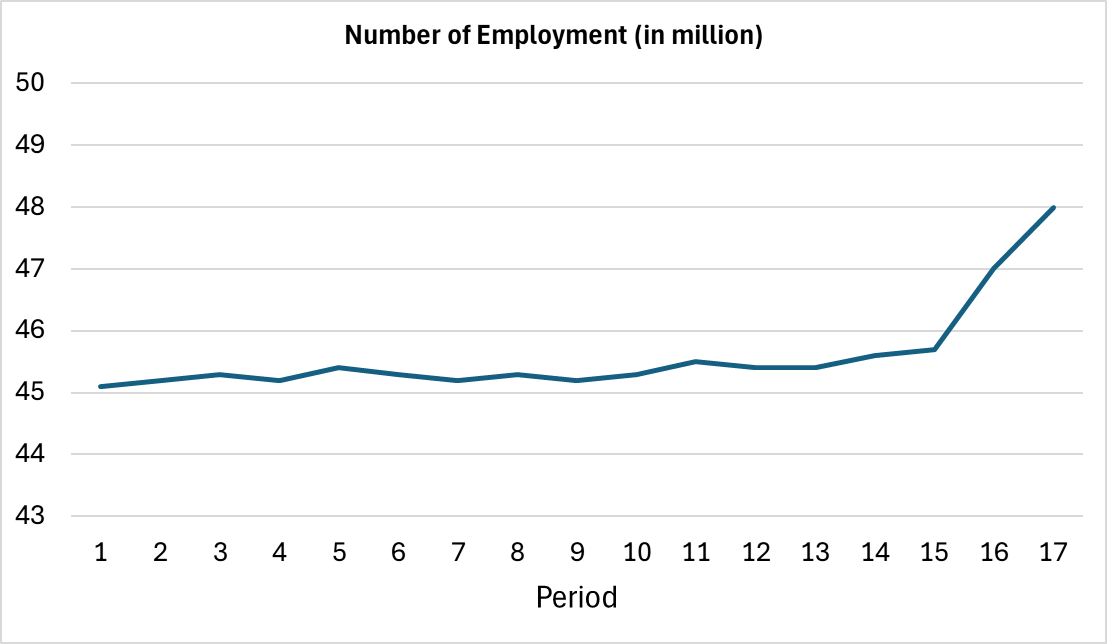
\includegraphics[width=0.7\linewidth]{figure/fig1}
\end{figure}

\begin{figure}[htbp!]
	\centering
	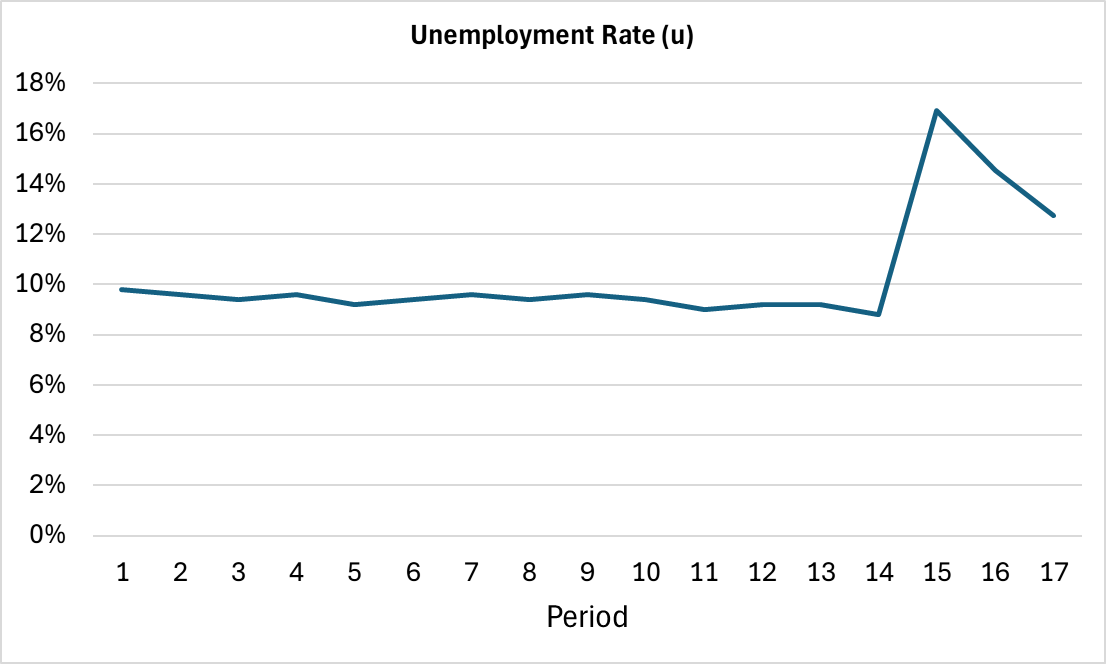
\includegraphics[width=0.7\linewidth]{figure/fig2}
\end{figure}


Let \( E \) represent the number of employed individuals, \( U \) the number of unemployed individuals, $L$ the number of labour force, and \( u \) the unemployment rate.

\clearpage

\begin{enumerate}[label=(\alph*)]
	\item \textbf{(2 pts)} How can the unemployment rate $u$ and labour force $L$ be defined in terms of the symbols given above?

	\item \textbf{(3 pts)} Why does the unemployment rate experience a sharp increase in period 15? Explain using the definition provided above.

	\item \textbf{(5 pts)} Given the conclusion you have in part b), trace a rough graph of the number of labour force and the number of unemployment over time.
\end{enumerate}

\clearpage
\textbf{Solution}
\begin{enumerate}[label=(\alph*)]
	\item 
	\[u = \frac{U}{L}\]
	\[L = U+E\]
	\item By using the definition above,
	\[u = \frac{U}{L}\]
	The only way for this to increase is through an increase in \( U \). However, we observe that total employment (\( E \)) remains unchanged in period 15 and increases afterward. This implies that \( L \) must also increase as a result, given that \( L = U + E \).
	\item 
	*The labour force would have a shape rise in period 15. After that, there could be flat (like in the graph below), and slightly moving up or down as well.
	\begin{figure}[htbp!]
		\centering
		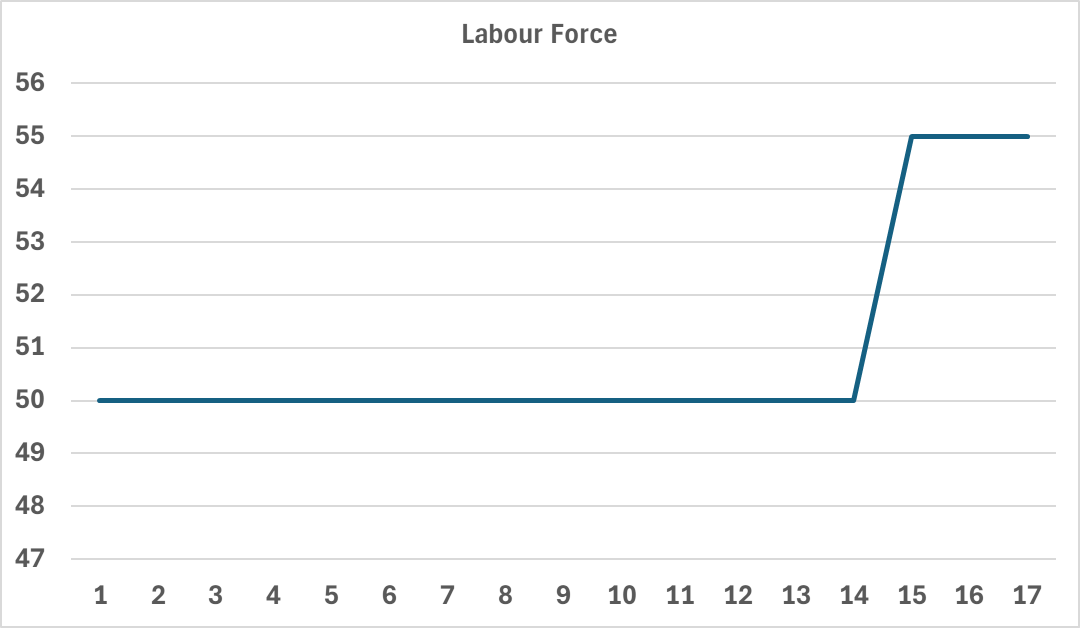
\includegraphics[width=0.7\linewidth]{figure/fig3}
	\end{figure}
	
	
	\begin{figure}[htbp!]
		\centering
		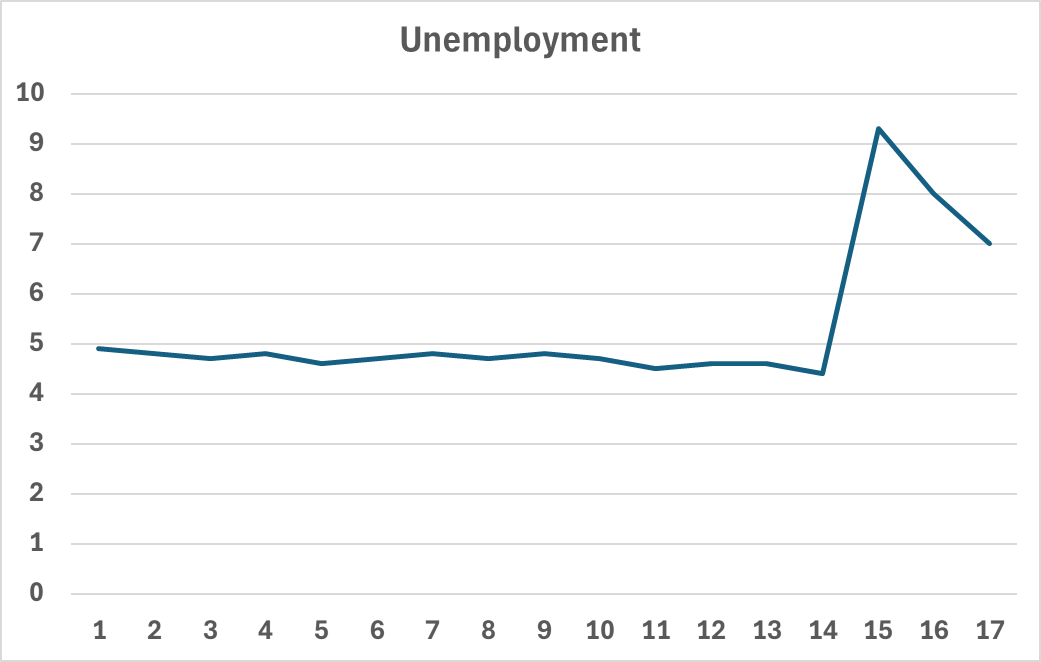
\includegraphics[width=0.7\linewidth]{figure/fig4}
	\end{figure}
	
	*If the labour force figure shown a upward trend after period 15, the unemployment may not fall to match with the unemployment rate figure.
\end{enumerate}

%\newpage
%\begin{center}
%	This page intentionally left blank. Please continue your answer for q.2 below.
%\end{center}
%\vspace*{\fill}

\newpage


\clearpage

\item  \textbf{(35 pts)}\label{P4}  This question relates to the combined Romer and Solow  growth model discussed in Chapter 6. Alton, a closed economy without government spending, features a production function:

\[Y_t = A_t^{3/4} K_t^{1/3} L_{y,t}^{2/3}\]

Here, \(Y_t\) represents the output, \(K_t\) denotes the capital, \(L_{y,t}\) stands for the labour employed and $A_t$ stand for TFP (or stock of ideas) in period \(t\). Alton's capital accumulation follows the standard function:

\[K_{t+1} = (1 - \delta) K_t + I_t\]

In this equation, \(\delta\) represents the depreciation rate, and \(I_t\) represents the investment in period \(t\). The accumulation of ideas  following:

\[\Delta A_{t+1} = \bar{z}L_{a,t}\]
where $\bar{z}$ is the productivity of idea creation.

The sum of numbers of workers ($L_{y,t}$) and researchers ($L_{a,y}$) equal to the total population: $L_{y,t} + L_{a,t} = N_t$.  The labour supply is inelastic, with the economy consistently providing \(N_t\) units of labour at any given wage.  The population is growing at the rate of $\bar{n}$. Meanwhile, there are $\ell$ proportion of the population work in the idea production. Alton's population save a proportion \(\bar{s}\) of their output for investment each period.

\begin{enumerate}[label=(\alph*)]
	\item \textbf{(3 pts)} Convert the production to intensive form.

	\item \textbf{(2 pts)} Convert the formula in part a) into the growth rate. 

	\item \textbf{(4 pts)} Show and discuss why the growth rate of output per capita ($g_y$) and capital per capita ($g_k$) are equal on the balance growth path? 


	\item \textbf{(4 pts)} Show that the growth rate of ideas $g_A$ is determined by constants on the balance growth path.
	\clearpage
	
	\item \textbf{(3 pts)} Express $g_y$ as a function of $g_A$ on the balance growth path. 

	\item \textbf{(3 pts)}  Find the balanced growth path of \textit{output per worker} as a function of $A_t$ and other exogenous variables and parameters.
	
	\item \textbf{(4 pts)} The Alton government is considering implementing measures such as low-cost childcare and tax credits to encourage population growth, as the current total fertility rate has reached an all-time low.
	
	Draw the transition in output per person from the balanced growth path before the policy change to after the policy change. Label all axis and key points of interest. Provide a explanation in 3-4 sentences.
	
	\item \textbf{(12 pts)} (separate from part g)  A portion of Alton's population consists of refugees from a neighboring country. These refugees have fully integrated into Alton's economy, contributing to the workforce in both the research and production sectors in the same proportions as Alton's native population. At period \( T \), the war ends, and half of the refugees decide to return to their home country ($\ell$ proportion of them are in the idea sector).	
	
	 Draw the transition in \textit{population}, \textit{output per person} and \textit{total consumption} from the balanced growth path before the policy change to after the policy change. Label all axis and key points of interest. Provide a explanation in 3-4 sentences.
	
%	\clearpage
%	\begin{center}
%		This page intentionally left blank. Please continue your answer below.
%	\end{center}
%	\vspace*{\fill}

\end{enumerate}

\clearpage
\textbf{Solution}
\begin{enumerate}[label=(\alph*)]
	\item  
	Divide the production function by $N$ and use $L_{a,t} = (1-\ell) \bar{N} \implies $
	 \[\frac{Y_t}{N_t} = y_t= A_t^{3/4} \frac{K_t^{1/3} L_{y,t}^{2/3}}{N_t^{1/3} N_{t}^{2/3}}  \]
	 \[y_t= A_t^{3/4} k_t^{1/3} (1-\ell)^{2/3}\]

	\item 
		\[
		g_{yt} = \frac{3}{4} g_{At} + \frac{1}{3} g_{kt} 
		\]
		
	\item 
	
	Plug in $I_t = s Y_t$
	\[K_{t+1}- K_t = \Delta K_{t+1}=  sY_t -\delta K_t\]
	Divide both side by $K_t$,
	\[\frac{\Delta K_{t+1}}{K_t} = g_K  = s\frac{Y_t }{K_t}-\delta = s\frac{Y_t/L_t }{K_t/L_t}-\delta = s\frac{y_t }{k_t}-\delta\]
	Now, recall that $k_t = \frac{K_t}{L_t}$ and apply the growth rate approximate formula:
	\[g_k = g_K - g_L\]
	
	Next, plug in the $g_K$ above and the fact that $g_L = \bar{n}$
	\[g_k= \frac{\Delta k_{t+1}}{k_t} = s\frac{y_t }{k_t}-\delta - \bar{n}\]

	
	On the BGP, \(g_{k,t}\) is a constant, therefore, the right-hand side must also be constant. Given that \(\bar{s}\) $\bar{n}$ and \(\delta\) are constants, \(\frac{y_t}{k_t}\) must be constant. This condition is met only if \(y_t\) and \(k_t\) are growing at the same rate. If \(y_t\) were growing at a faster rate, the ratio \(\frac{y_t}{k_t}\) would increase each period. Therefore, it follows that \(g_k^* = g_y*\).
	
	\vspace{1cm}
		
		
	\newpage
	\item \textbf{(3 pts)} 	
	Researchers are used to produce new ideas:
	\[g_{At} = \frac{\Delta A_{t+1}}{A_t} =\frac{\bar{z}L_{a,t}}{A_t} \]
	Rearrange the the formula,
	\[A_t = \frac{1}{g_{A,t}} \bar{z} L_{a,t}\]
	On  the BGP, $g_{At} = g^*_{At}$, therefore, only the term $L_{a,t}$ is a variable. Apply the growth rate formula,
	
	\[g_{A,t} = g_{La} = \bar{n}\]
	
	Now, we know that $g_{At}$ is a constant.
	
	
	\item \textbf{(3 pts)}	
	Plug in $g_{At}=\bar{n}$, $g_K^* = g_Y^*$ into the $g_y$ equation above
	\[g_{y}^* = \frac{3}{4}\bar{n} + \frac{1}{3} g_{y}^* \implies g_{y}^* = \left(\frac{3}{2}\right) \left(\frac{3}{4}\right)\bar{n} = \frac{9}{8} \bar{n}\]
	For the long-run combined model, this equation pins down	the growth rate of output and 	the growth rate of output per person
	
	*Either using $\bar{n}$ or $g_A$ is fine.
	
	%	\item \textbf{(3 pts)} Express $g_T$ as a function of $g_A$ on the balance growth path. 
	%	\vspace{1cm}
	
	
	%	\item \textbf{(3 pts)} 
	%	
	\vspace{1cm}
	
	\clearpage
	\item \textbf{(4 pts)} 
	Use the growth rate equation derived earlier. 
	Now, we know that $g_y^*$ is a constant along a balanced growth path. This implies
	\[\frac{k^*_t}{y^*_t} = \frac{\bar{s}}{g_y^* + \delta + \bar{n}}\]
	
	Rearrange and plug it this : $k^*_t  = \frac{\bar{s}}{g_y^* + \delta + \bar{n}} y^*_t$ into the production function:
	
	\[y_t^*= A_t^{3/4} \left(\frac{\bar{s}}{g_y^* + \delta + \bar{n}} y^*_t\right)^{1/3} (1-\ell)^{2/3}\]
	\[\implies y_t^{*}= \left[A_t^{3/4} \left(\frac{\bar{s}}{g_y^* + \delta + \bar{n}} \right)^{1/3} \right]^{3/2} (1-\ell) = A_t^{9/8} \left(\frac{\bar{s}}{g_y^* + \delta + \bar{n}} \right)^{1/2}  (1-\ell) \]
	
	\vspace{1cm}
	\item In this scenario, the government policy would result in an increase in \( \bar{n} \). This increase in \( \bar{n} \) would lead to a higher growth rate for both \( g_y \), causing the slopes of BGP of \( y \) to become steeper than before. However, the new balanced growth path (BGP) would be initially below the original BGP for a certain period because both \( g_y \) and \( \bar{n} \) have increased. Over time, the new BGP would surpass the old BGP and ultimately rise above it, as \( A_t \) grows at a faster rate.  In the graph, we assume that the growth from the increase in $\bar{n}$ outpace the slowdown from the other variables (e.g., $g_k$). 
	
	\begin{figure}[htbp!]
		\centering
		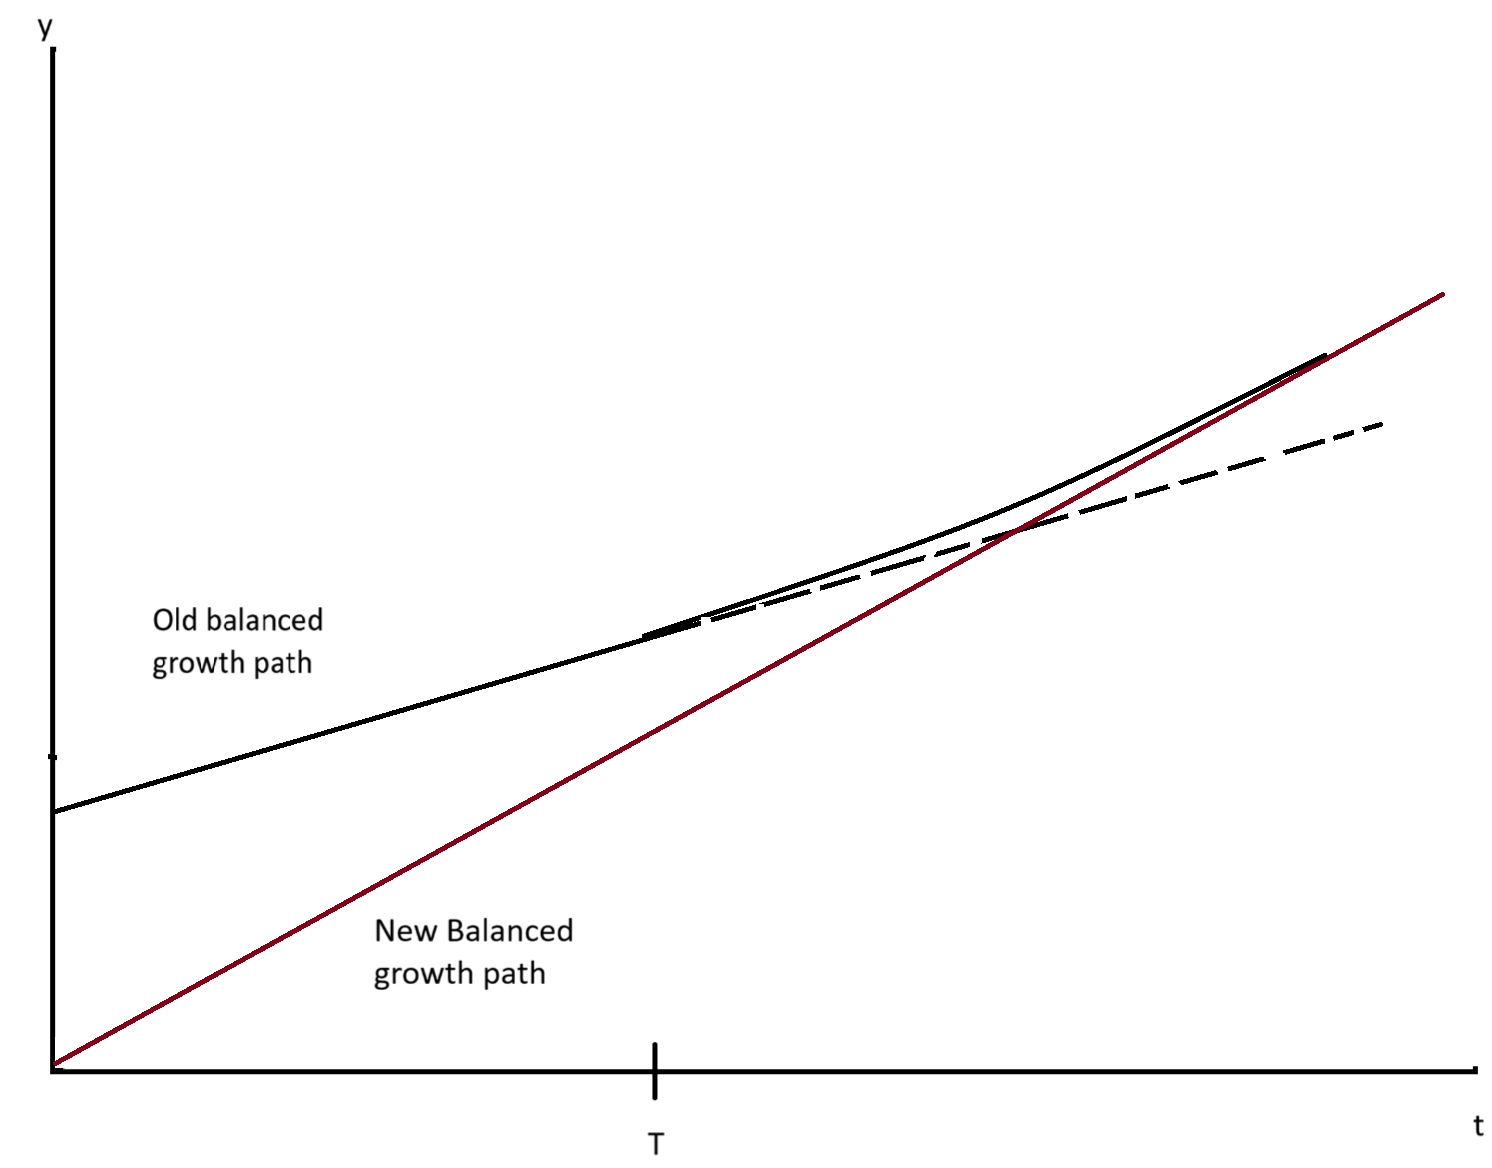
\includegraphics[width=0.45\linewidth]{figure/q6f}
	\end{figure}
	
%	\begin{figure}[htp!]
%		\centering
%		\includegraphics[width=0.7\linewidth]{figure/q6e}
%	\end{figure}
	
	\clearpage
	\item In this case, the $N$ falls right away and it doesn't distort the proportion of worker in the idea and in the production sector. Since the $\bar{n}$ did not change, there is a discrete fall at period T but the slope is unchanged. Due to this, the total output would fall, but the output per capita would go the opposite direction. The output capita $y_t= A_t^{3/4} k_t^{1/3} (1-\ell)^{2/3}$ would rise because $k$ increase as a result of fall in population. Therefore, we see a discrete jump in $y_t$. However, there would be a drop in total consumption $C=(1-s)Y$ at Period T since the total output is a function of $L_y$ which fall as a result of people moving out the country. The slope of the BGP is unchanged for all three variables. The BGP for $y$ would shift downward as a result of the decrease in $A$ due to the decrease in $N$ as the economy adjusting its $k$. Similar effect for the total consumption (recall that $C = (1-s)Y = (1-s)yN$. 
	
	Initially, the growth rates of \( y \) and \( Y \) would be lower because both \( g_A \) and \( g_k \) decrease. The decline in \( g_k \) occurs because \( y_t/k_t \) decreases as the population falls, given that $	\frac{y_t}{k_t} = \frac{A^{3/4} (1-\ell)^{2/3}}{k_t^{2/3}}$. Meanwhile, \( g_A \) decreases due to a smaller population size relative to its stock of ideas.
	
	In the graph, this is illustrated by a case where the growth rate turns negative (if \( y/k \) is sufficiently low, \( g_k \) can become negative), then gradually increases and converges to the balanced growth path (BGP). However, growth does not necessarily have to turn negative; as long as the growth rate slows down initially and then accelerates toward the BGP, the path is valid.
	
	
	
	
	\begin{figure}[htbp!]
		\centering
		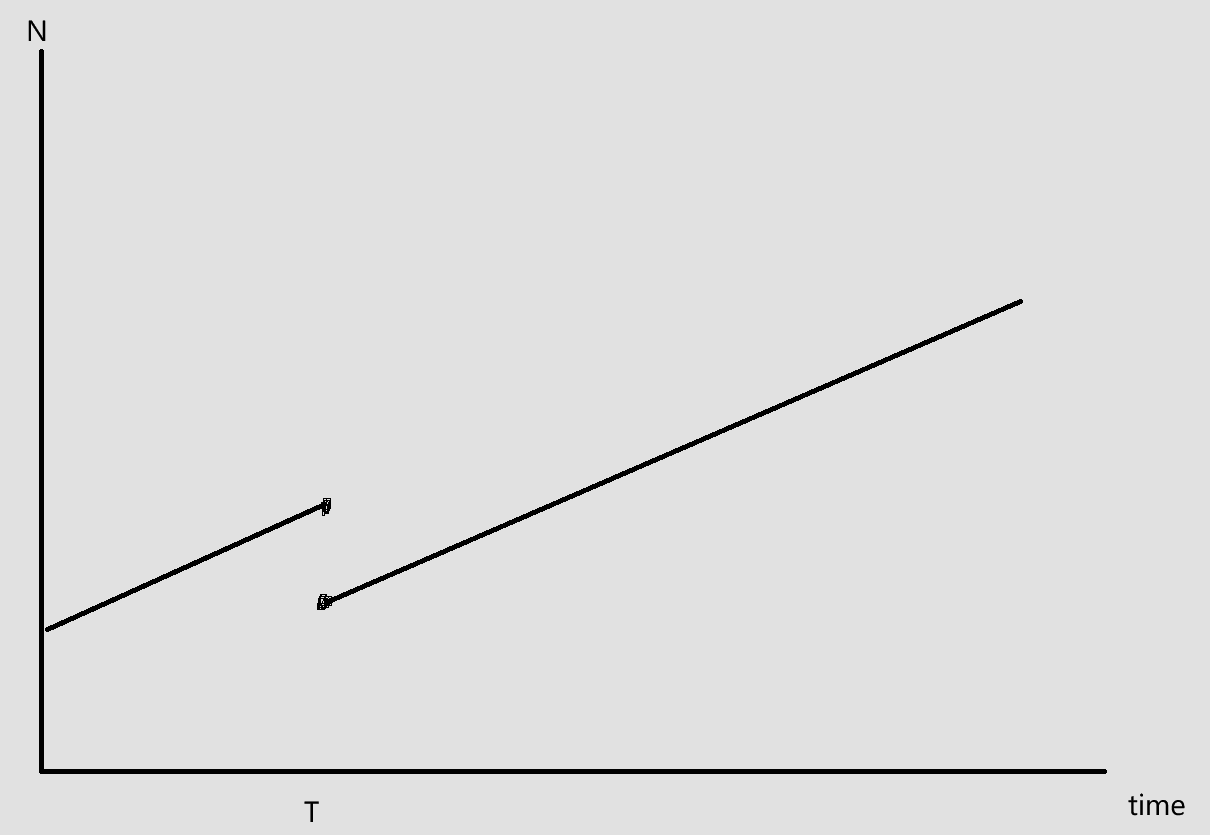
\includegraphics[width=0.7\linewidth]{figure/Q4-1}
	\end{figure}
	
	\begin{figure}[htbp!]
		\centering
		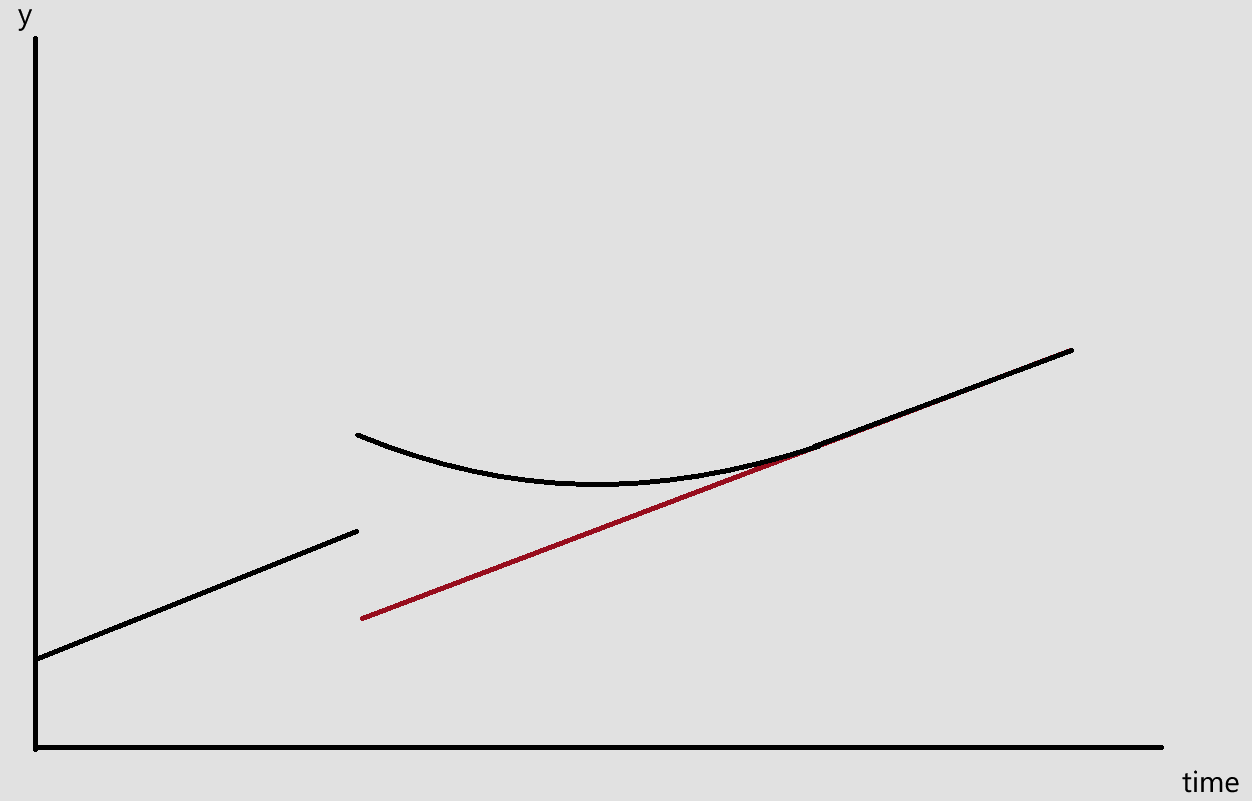
\includegraphics[width=0.7\linewidth]{figure/Q4-2}
	\end{figure}
	
	\begin{figure}[htbp!]
		\centering
		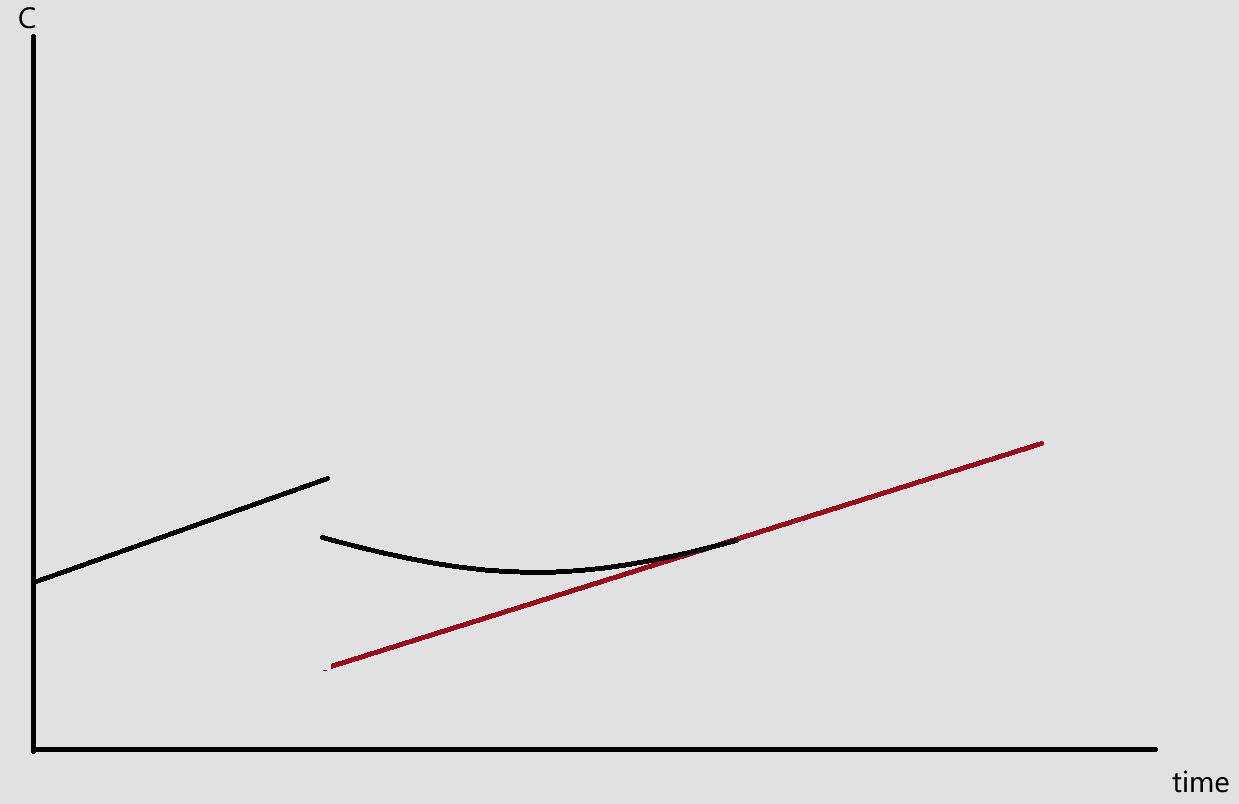
\includegraphics[width=0.7\linewidth]{figure/Q4-3}
	\end{figure}
	
	
\end{enumerate}

\newpage
\begin{center}
	This page intentionally left blank. Please continue your answer below.
\end{center}
\vspace*{\fill}
%
%\newpage
%\begin{center}
%	This page intentionally left blank. Please continue your answer below.
%\end{center}
\vspace*{\fill}

\centering{-- The End -- }
\end{enumerate}
  \end{document}
